\documentclass[a4paper,11pt]{extarticle}

\usepackage[default]{comfortaa}
\usepackage[utf8]{inputenc}
\usepackage[T1]{fontenc}
\usepackage[english]{babel}
\usepackage[left=0cm, right=0.5cm, bottom=0.5cm, top=0.5cm]{geometry}
\usepackage{fixltx2e}
\usepackage{graphicx}
\usepackage{amsmath}
\usepackage{amssymb}
\usepackage{mathrsfs}
\usepackage{indentfirst}
\usepackage[shortlabels]{enumitem}
\usepackage[usenames,dvipsnames]{xcolor}
\usepackage{tcolorbox}
\usepackage{marvosym}
\usepackage{genealogytree}
\usepackage{hyperref}
\usepackage{fontawesome}

%\colorlet{bgcol}{LimeGreen!40!white}
\colorlet{bgcol}{LimeGreen}
\newcommand{\circb}[1]{\begin{minipage}{1cm}
    \begin{tcolorbox}[colback=Green,colframe=Green,
        halign=flush center, valign=center, square, circular arc,
        width=0.8cm, left=0cm, right=0cm]
        {\large #1}
    \end{tcolorbox}
\end{minipage}}
\newcommand{\cvtitle}[1]{
    \begin{tcolorbox}[colback=bgcol,colframe=ForestGreen,
        height=1cm, valign=center, sharp corners=downhill]
        {\Large #1}
    \end{tcolorbox}
}
\newcommand{\gritem}{\color{bgcol}$\blacksquare$}
\renewcommand{\labelitemi}{\gritem}
\newcommand{\griitem}{\color{bgcol}$\blacktriangleright$}
\renewcommand{\labelitemii}{\griitem}
\newcommand{\myspace}{{\color{LimeGreen}\dotfill}}

\renewcommand{\wp}[1]  {\begin{minipage}[b][2mm][c]{3mm} #1 \end{minipage}}
\colorlet{skcol}{OliveGreen}
\colorlet{noskcol}{LimeGreen}
\newcommand{\skdabb} {\colorbox{ForestGreen!80!white}{\color{skcol}$\blacksquare$~\color{noskcol}$\blacksquare$~\color{noskcol}$\blacksquare$}}
\newcommand{\skmore} {\colorbox{ForestGreen!80!white}{\color{skcol}$\blacksquare$~\color{skcol}$\blacksquare$~\color{noskcol}$\blacksquare$}}
\newcommand{\skexp}  {\colorbox{ForestGreen!80!white}{\color{skcol}$\blacksquare$~\color{skcol}$\blacksquare$~\color{skcol}$\blacksquare$}}

\newcommand{\lang}[2]{\hfill \textsc{\scriptsize #1, \textasciitilde#2Sloc}}
\newcommand{\director}[1]{\hfill {\scriptsize #1}}

\begin{document}

\begin{minipage}[c]{0.35\linewidth}
    \begin{tcolorbox}[
        colback=bgcol,
        colframe=ForestGreen,
        subtitle style={
            colback=bgcol,
            coltext=black
        },
        leftrule=2mm,
        sharp corners=uphill,
        height=282mm,
    ]
        \begin{minipage}{0.45\linewidth}
            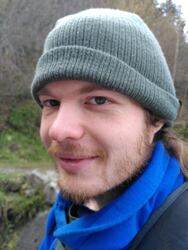
\includegraphics[width=\linewidth]{head.jpg}
        \end{minipage}
        \hfill
        \begin{minipage}{0.45\linewidth}
            Luc

            \textbf{Chabassier}
        \end{minipage}

        \vspace{0.2cm}
        {\small
        \circb{\gtrsymBorn} September 19, 1996 \newline
        \circb{\Telefon} +33~(0)609642210 \newline
        \circb{\Letter} \href{mailto:luc.chabassier@ens.fr}{luc.chabassier@ens.fr} \newline
        \circb{\Mundus} \href{https://dwarfmaster.net}{dwarfmaster.net} \newline
        \circb{\faGithub} \href{https://github.com/dwarfmaster}{dwarfmaster} \newline
        }

        \vspace{0.3cm}
        \tcbsubtitle{\Large\bf About me}

        A student in computer science, passionate with everything related to
        computers, who started programming for fun at the age of 14. Leaving
        the imperative paradigm he started with, he now focus mostly on
        strongly typed functional languages and formal proofs.

        \vspace{0.3cm}
        \tcbsubtitle{\Large\bf Interests}

        Programming, reading science fiction and fantasy, bouldering and hiking.

        \vspace{0.3cm}
        \tcbsubtitle{\Large\bf Skills}
        \begin{description}\setlength{\itemsep}{0em}
          \item[C++]\hfill\skexp
          \item[Haskell]\hfill\skexp
          \item[\LaTeX]\hfill\skexp
          \item[Linux]\hfill\skexp
          \item[Coq]\hfill\skmore
          \item[Prolog]\hfill\skmore
          \item[Nix]\hfill\skmore
          \item[OCaml]\hfill\skdabb
          \item[Python]\hfill\skdabb
        \end{description}

        \vspace{0cm}
        \tcbsubtitle{\Large\bf Languages}

        Native french, fluent english, basic spanish


    \end{tcolorbox}\end{minipage}
    \hfill
    \begin{minipage}[c][282mm][t]{0.60\linewidth}

        \cvtitle{Education}

        \begin{itemize}
          \item \emph{Pierre de Fermat} in Toulouse:
                \begin{itemize}
                  \item \textbf{2014} baccalauréat S with highest honours
                  \item \textbf{2014-2016} Maths-Physic preparatory class
                \end{itemize}
          \item \emph{École Normale Supérieure} in Paris:
                \begin{itemize}
                  \item \textbf{2016-2017} Computer science bacherlor's degree
                  \item \textbf{2017-2018} First year of computer science master's degree
                  \item \textbf{2018-2019} Mathematics bahelor's degree
                  \item \textbf{2020-2021} MPRI: Second year of computer science master's degree \emph{(unfinished)}
                \end{itemize}
        \end{itemize}

        \cvtitle{Research Experiences}

        \begin{itemize}
          \item \emph{\small (2017)} \textbf{2 months Internship}
                \lang{$\lambda$Prolog}{1k}\\
                A deriving mecanism for Coq
                \director{Enrico Tassi} \\
                MARELLE team at INRIA Sophia-Antipolis
          \item \emph{\small (2018)} \textbf{5 months Internship}
                \lang{CL/Haskell/C++}{3k}\\
                Infering frames semantics
                \director{Marie-Claude L'Homme}\\
                Département de linguistique à UdeM
          \item \emph{\small (2019)} \textbf{\href{https://github.com/dwarfmaster/memoire-dma-l3}{Maths dissertation}}
                \lang{\LaTeX}{4k}\\
                Category theoretic approach to CSPs
                \director{Damianno Mazza}
          \item \emph{\small (2021)} \textbf{4.5 months internship} \emph{(future)}
                \lang{Dedukti}{?}\\
                Encoding extensional type theories in Dedukti
                \director{Bruno Barras} \\
                Laboratoire de Méthodes Formelles at Inria Paris-Saclay
        \end{itemize}

        \cvtitle{Other Experiences}

        \begin{itemize}
          \item \emph{\small (2014)} \textbf{Project} \href{https://github.com/DWARVES/Project-Warrior}{Warrior}
                \lang{C++}{30k}\\
                A fighting game
          \item \emph{\small (2016)} \textbf{Project} \href{https://github.com/TWal/ENS\_Adac}{Adac}
                \lang{Haskell}{4k}\\
                A compiler for a subset of Ada
          \item \emph{\small (2017)} \textbf{Project} \href{https://github.com/lucas8/absint}{Absint}
                \lang{Haskell}{1k}\\
                Abstract interpreter for a subset of C
          \item \emph{\small (2018)} \textbf{Presentation} \href{https://sapt.fr/exposes/verification-automatique-de-preuves-884}{Vérification de preuve}
                \lang{\LaTeX}{2k}\\
                Popularization of some proof theoretic results
          \item \emph{\small (2019-2020)} \textbf{5.5 months internship}
                \lang{C++}{5k}\\
                Analysis of code using web frameworks in \href{https://labs.oracle.com/pls/apex/f?p=LABS:project_details:0:13}{Parfait}\\
                ORACLE labs in Brisbane
          \item \emph{\small (2020)} \textbf{Project} \href{https://github.com/dwarfmaster/free_group_coq}{Free Group}
                \lang{Coq}{1k}\\
                Formalisation of the free group construction
          \item \emph{\small (2020)} \textbf{Project} \href{https://github.com/math-fehr/Untitled-Language}{Untitled Language}
                \lang{Haskell}{2.5k}\\
                A functional programming language with linear types
        \end{itemize}

    \end{minipage}

\end{document}

